% $Id$
% vim: tw=78 ai spell spelllang=en

\documentclass[10pt]{llncs}
\usepackage{color}
\usepackage{url}
\usepackage{xspace}
\usepackage{graphicx}
\usepackage{listings}

%{{{ LaTeX definitions

\newcommand\Color[2]{\textcolor{#1}{#2}}
\newcommand{\nb}[1]{\marginpar{\scriptsize #1}}
\renewcommand\note[1]{\nb{\Color{blue}{#1}}}
\newcommand\todo[1]{\nb{\Color{red}{#1}}}

\newcommand{\Stanse}{\textsc{Stanse}\xspace}
\newcommand{\TC}{\textsc{ThreadChecker}\xspace}
\newcommand{\AC}{\textsc{AutomatonChecker}\xspace}
\newcommand{\RC}{\textsc{ReachabilityChecker}\xspace}

\lstset{tabsize=2,numbers=none,showstringspaces=false,breaklines=true,
        breakatwhitespace=true,escapeinside={(*@}{@*)},
	basicstyle=\scriptsize}

%}}}

\begin{document}

%{{{ Title+Authors+Abstract

\title{{STANSE}: Bug-finding Framework\\ for C Programs}
\author{Jan~Obdr\v{z}\'alek, Ji\v{r}\'\i~Slab\'y and Marek~Trt\'{\i}k}
\institute{Faculty of Informatics, Masaryk University, Brno, Czech Republic
\email{\{obdrzalek,slaby,trtik\}@fi.muni.cz}}

\maketitle

\begin{abstract}
  \Stanse is a free (available under the GPLv2 license) modular framework
  for finding bugs in C programs using static analysis. Its two main design
  goals are applicability on large software projects like Linux kernel and
  extendability with new bug-finding techniques with a minimal effort.
  % Above that the reported results can be presented in multiple ways, web
  % included.
  Currently there are three bug-finding algorithms implemented within
  \Stanse: \AC checks properties described in an automata-based formalism,
  \TC detects deadlocks among multiple threads, and \RC looks for
  unreachable code. \Stanse has been tested on the Linux kernel, where it
  has found dozens of previously undiscovered bugs.
\end{abstract}

%}}}

%{{{ Intro

\section{Introduction}
\label{sec:introduction}

During the last decade, bug-finding techniques based on static analysis have
finally come of age. One of the papers to really stir interest
was~\cite{ECCH00}, showing that static analysis can efficiently find many
interesting bugs in a real-world code.
%, as demonstrated on the Linux kernel. 
This work eventually led to a successful commercial tool called
\textsc{Coverity}~\cite{coverity}. Over the years, several other successful
tools, like \textsc{CodeSonar}~\cite{codesonar} or
\textsc{Klocwork}~\cite{klocwork}, appeared.
%
However, such fully-featured tools are neither free to obtain, nor is their
code available (e.g.~for developing new algorithms or tailoring the existing
tools to specific tasks). The existing free tools are usually severely
limited in what they can do (e.g.~\textsc{Uno}~\cite{uno},
\textsc{Sparse}~\cite{sparse}, \textsc{Smatch}~\cite{smatch}). One notable
exception is \textsc{FindBugs}~\cite{HP04,findbugs}, a successful tool
working on Java code.
%
\Stanse is intended to fill this gap for C language. It can be seen in
two ways:
\begin{enumerate}
\item \Stanse is a robust framework (written predominantly in Java) for
  implementing diverse static analysis algorithms. An implemented algorithm
  can be immediately evaluated on large real-world software projects written
  in C as the framework is capable to process such projects (for example, it
  can process the whole Linux kernel). An implementation of such an algorithm
  within the framework is called \emph{checker}.

  \item As \Stanse contains three checkers already, it can be also seen as a
  working static analysis tool.
\end{enumerate}

The rest of the paper is structured as follows. Section~\ref{sec:framework}
describes the functionality provided by the framework, while
Section~\ref{sec:checkers} is devoted to the three existing checkers.
Section~\ref{sec:results} presents some results of \Stanse on the Linux
kernel. The last section summarizes the basic strengths of \Stanse and
mentions some directions of its future development.

%}}}
%{{{ Framework

\section{Framework Functionality}
\label{sec:framework}

The functionality provided by the \Stanse framework can be roughly separated
into several stages. First, the framework reads in the configuration
including the list of source files to be analysed and checkers to be
used. The source files are then parsed into a set of \emph{internal
  structures}, namely \emph{abstract syntax trees (ASTs)},
\emph{control-flow graphs (CFGs)}, and \emph{call-graphs}. Next, checkers
are run on these structures and error reports are collected and presented.

\subsection{Selecting and Parsing Source Files}

There are several ways to tell \Stanse what source files to analyse. Besides
the standard possibilities (a single given file, all files from a given
directory, all files listed in a given file), \Stanse can also derive all
the necessary information from a project \textsf{Makefile}. In this case,
\Stanse also remembers compiler flags for preprocessing purposes. This
functionality is inspired by the \textsc{Sparse}~\cite{sparse} tool.
%  but differs in that it generates the file
% list only once so the build needs not be run over and over for verification
% runs e.g. with different configuration like distinct checkers.

\Stanse can process source files written in C, more specifically the
ISO/ANSI C99 standard and most of the GNU C extensions.
Before parsing, the sources are preprocessed by the standard GNU C
preprocessor.
%  We are currently working on support of
% other languages, in particular C++.
%
The code is then parsed into the mentioned internal structures: a
call-graph, a CFG for each function, and an AST for each code piece
corresponding to a node of some CFG.
% These structures are linked in a natural way.
All these structures can be dumped in a textual or graphical form.

As mentioned earlier, the design of the framework is geared towards
analysing large software projects. Such projects consist of hundreds or
thousands of modules (compilation units). In practice, it is often
impossible to store all the corresponding internal structures in the
memory. The \Stanse framework therefore applies automatic \emph{streaming}
of the internal structures, currently on a module basis.
%
Instead of parsing all source modules at the beginning, a module is streamed
in only when \Stanse needs to access some internal structure corresponding
to the module. In other words, the internal structures are constructed in a
lazy manner.
% It means not everything is parsed at the start of the checking
% process. Hence it is not a time or memory bottleneck at that time.
%
If the memory occupied by internal structures exceeds a given limit, some
internal structures have to be freed before another module is streamed
in. The structures to be freed are selected by an LRU (least-recently-used)
approach: \Stanse discards all internal structures of the module whose
structures are not accessed for the longest time. If the discarded structure
is later accessed again, the corresponding module is streamed back in. Both
laziness of internal structures and streaming are completely invisible to
checkers.

\subsection{Traversing the Parsed Code}\label{ssec:travers}

Although a checker can process the internal structures in an arbitrary way,
most of checkers walk through CFGs using some standard strategy. To prevent
unnecessary reimplementations, the most important and heavily used traversal
methods are implemented directly inside the framework. With this
functionality, one can implement a new checker (or its part) by specifying
\begin{itemize}
\item whether it should go through CFGs forwards or backwards, breadth-first
  or depth-first,
\item if the interprocedural walk-through should be performed or not (if
  not, the function calls are ignored), and
\item a method (callback) to be called for each visited node in a CFG.
\end{itemize}
This makes implementation of new algorithms extremely simple.

\subsection{Processing Errors}

\begin{figure}[t]
  \centering
    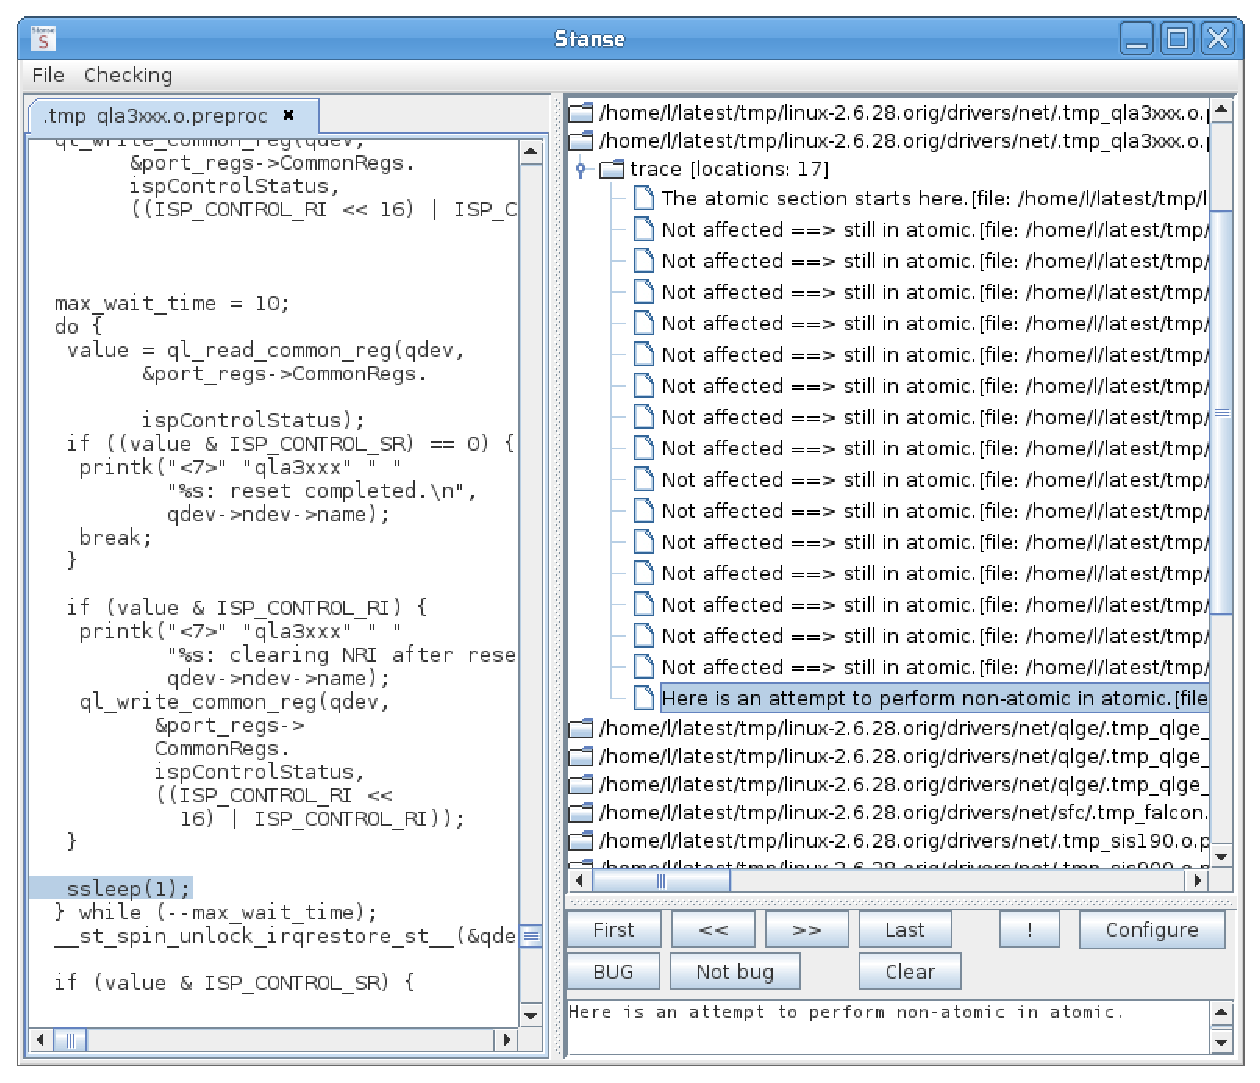
\includegraphics[width=9.1cm]{screen-bug-tracing}
  \caption{The error trace GUI browser.}
  \label{fig:bugtrace}
\end{figure}

Once a checker finds an error, it reports back a commented \emph{error
  trace} (a path in the analysed code) demonstrating this error. 
% \Stanse provides support for grouping together error traces representing the same kind of error
% and leading from/to the same point. 
\Stanse provides several possibilities to present the error traces: they can
be printed to the console, displayed using a built-in error trace GUI
browser (see Figure~\ref{fig:bugtrace}), or saved to an external file in XML
format. This XML file has a wide variety of possible applications. For
example, we supply a tool transforming the XML file into an \textsc{SQLite}
database complemented with a web interface allowing to browse errors in the
database via a web browser. Using the web browser or the built-in error GUI
browser, one can mark errors as real bugs or false-positives. \Stanse
also provides various statistics of errors like number of errors per file
and checker, frequency of errors of the same kind, percentage of
false-positives (based on user feedback), etc.


% \note{Tady to zni, jako by
%   soucasti \Stanse byl i ten web interface. Co presne dela ten creator?
%   Nestaci napsat ``For example, we supply a tool translating the XML file
%   into an \textsc{SQLite} database.''?}\todo{JS: Taky, ze ano, primitivni,
%   ale je :). Viz \url{http://decibel.fi.muni.cz/~xslaby/stanse/}. Creator
%   dela presne ten preklad XML do db, jak pises v te vete.}

\subsection{Other Features}

The framework provides some other features. For example, it supports
parallel execution of more checkers (in threads). Note that the internal
structures are shared by all running checkers. Further, \Stanse can run in a
command line mode or via a fully featured GUI. If properly configured,
\Stanse can be used as a ``push-the-button'' tool. Due to the design of the
framework, \Stanse can be adapted to handle other programming languages by
writing appropriate parsers. Finally, the \Stanse framework is basically a
Java library, so it can be easily transformed into a static analysis plug-in
for some IDE (e.g.~Eclipse or NetBeans).

%}}}
%{{{ Checkers

\section{Checkers}
\label{sec:checkers}

% Each checker is a module which, with the support of the \Stanse framework,
% implements some verification technique (e.g. deadlock detection). There can be
% many different checkers running simultaneously (either in parallel or
% sequentially) in \Stanse at any given time. They all run independent of each
% other.

% A new checker, in order to be used with \Stanse, needs just to implement the
% general checker interface mentioned above and register with the framework.
% Users need not to implement their checkers if they don't want to. Instead,
In this section we describe the three currently available checkers.

\subsubsection{\AC}
is heavily influenced by~\cite{ECCH00}. It takes, as an input, a set of
finite-state automata that describe some properties which we want to check.
Properties like locking discipline, interrupt management, null pointer
dereference, dangling pointers and many others can be handled this way.

Compared to the implementation described in~\cite{ECCH00} and~\cite{HCXE02},
our technique differs in several aspects. In particular, we do not use
metacompilation, automata are not input-language specific (a pattern
matching is used instead), and
% our analysis is path-sensitive on checker level, but for this reason
the interprocedural analysis is done in the context of a single input file.

% The patterns in the configuration are specified in the same language as AST is
% represented, so currently in XML. The idea behind was to isolate the patterns
% from the source code.

\subsubsection{\TC}
aims to check for possible deadlocks in concurrent programs. The technique
is based on the notions of locksets of~\cite{relay} and deadlock detection
by looking for cycles in \emph{resource allocation graphs (RAGs)}. \TC first
tries to identify the parts of the code which can run in parallel, as
different threads. Then it builds a set of \emph{dependency graphs} for each
such a thread. A dependency graph statically represents the possible
locksets during one execution of a thread. Dependency graphs are then
combined and transformed to RAGs. If some RAG contains a cycle, an error is
reported.

\subsubsection{\RC}
searches CFGs for unreachable nodes. These are then reported as warnings or
errors, depending on importance (e.g. superfluous semicolons are less
important than unused branch). The primary goal of \RC is to demonstrate the
simplicity of a new checker implementation using the framework features
described in Subsection~\ref{ssec:travers}: the code of the checker has less
than 200 lines including the mentioned error/warning classification and many
strings and comments.

%}}}
%{{{ Results

\section{Results on Linux Kernel}
\label{sec:results}

We have several reasons to choose the Linux kernel to test \Stanse: the
kernel presents a large and freely available codebase, it fully exercises
most features of ISO/ANSI C99 and GNU C extensions, it is under constant
development (new bugs are appearing), and absence of bugs are of great
concern. 

We applied \Stanse with the three checkers described in the previous section
to kernel version 2.6.28. \AC uses three automata describing the following
kinds of errors:
\begin{itemize}
\item incorrect pairing of functions (imbalanced locking, reference
  counting errors)
\item bugs in pointer manipulation (null dereference, dangling pointers, etc.)
\item deadlocks caused by sleeping inside spinlocks or interrupt handlers
\end{itemize}

The running time of \Stanse on a common desktop machine with 2 cores and
4\,GiB of memory is under 100 minutes. The memory usage of the Java process
oscillates between 400 and 1000\,MiB. The number of errors reported by the
checkers can be found in Table~\ref{tab:results}. Let us note that \RC
actually detected 751 errors, but 720 of them are of a low importance
(including 696 superfluous semicolons) and they are omitted from our
statistics.

\begin{table}[b]
\begin{center}
\setlength{\tabcolsep}{3pt}
\begin{tabular}{|l|l|c|c|c|c|} \hline
\textbf{Checker} & \textbf{Automaton} & \textbf{Reported err.} & \textbf{Bugs} & \textbf{False pos.} & \textbf{Ratio} \\ \hline\hline
& Pairing           & 266 & 65  & 143 & 31.3\,\% \\ \cline{2-6}
\AC & Pointers        & 86  & 48  & 37  & 56.5\,\% \\ \cline{2-6}
& Deadlocks            & 35  & 16  & 18  & 47.1\,\% \\ \hline
\multicolumn{2}{|l|}{\TC}    & 20  & 9   & 11  & 45.0\,\% \\ \hline
\multicolumn{2}{|l|}{\RC}    & 31  & 31  & 0   & 100.0\,\%  \\ \hline\hline
\multicolumn{2}{|l|}{\textbf{Overall}}  & 438 & 169 & 209 & 44.7\,\% \\ \hline
\end{tabular}
\end{center}
\caption{\Stanse results on Linux kernel version 2.6.28.}
\label{tab:results}
\end{table}

We have manually analysed all the reported errors and mark them as real bugs
or false positives (with an exception of 60 errors reported by \AC where we
are not able to decide in a short time whether it is a false positive or
not). The numbers of real bugs, false positives and the ratio of real bugs
to all classified reported errors can be also found in
Table~\ref{tab:results}. The overall ratio of real bugs to all classified
errors is not high: 44.7\%. However, \Stanse in the current version does not
have any thorough false-positive filtering technique.

More than 70 of the 169 found bugs have been reported to kernel developers
and fixed in the following kernel releases (the other bugs have been
independently discovered and reported by someone else or the incorrect code
disappeared from the kernel before we finished our evaluation of reported
errors). Some of the reported bugs remained undiscovered for seven years
(for example, see \url{http://lkml.org/lkml/2009/3/11/380}). % This is
% despite the kernel being regularly checked by \textsc{Coverity}. We guess
% that it is due to a very restrictive false-positive filtering used.

We have reported another 50 bugs found by \Stanse in the subsequent versions
of the kernel. This number is increasing every month.

%}}}
%{{{ Conclusions

\section{Conclusions and Future Work}

\Stanse is a free Java-based framework for simple implementation of
bug-finding algorithms based on static analysis. The framework can process
large-scale software projects written in ISO/ANSI C99. \Stanse does not
currently use any new techniques -- its novelty comes from the fact that (to
our best knowledge) there is no other open-source framework with comparable
applicability and efficiency. \Stanse is available at
\url{http://stanse.fi.muni.cz}. 
%
We note that more than 130 bugs found by \Stanse have been reported
to and confirmed by Linux kernel developers already.

% Even if \Stanse with its three simple bug-finding algorithms has already
% found more than 130 real bugs in the Linux kernel and this number is growing
% every month, there are still many aspects that should be improved.

\subsubsection{Future Work}
We plan to improve the framework in several direction. We are currently
working on C++ support. Further, we plan to provide \Stanse in the form of a
plug-in for Eclipse and NetBeans IDEs. A lot of work can be done in the area
of automatic false-alarm filtering and error importance classification.
% We also plan to design and implement some difference analysis of results
% produced by \Stanse on various versions of the same software project.
Independently of new features development, we would like to speed up the
framework as well. More precisely, we intend to replace the current parser
written in Java by an optimized parser written in C, to replace the XML
format of internal structures by a more succinct representation, to add a
support for function summaries, etc.

% C++ support, rewrite to C, get rid of XML, daily analysis, results difference.
% Should this be here? Pay attention, we reference future work section above.

% ... but the parser itself is
% generated by \textsc{ANTLR} from a top-down C grammar which we developed
% based on provided example grammar. This is a limiting factor of the whole
% tool when parsing C sources, because (according to the \textsc{ANTLR}
% authors) the C parser in Java is unoptimized and slow -- this is not true
% for C parser in C, so we use it for parsing included headers to extract type
% definitions. The rest of file is handled in Java.

% Nowadays, we are working hard on merging a C++ support which is based on
% \textsc{clang++} from \textsc{LLVM} suite and we are almost finished. We do
% not use \textsc{clang} (at the time of writing this article, 2.8 is stable)
% for pure C because it still misses some features from the GNU C which are
% widely used in the Linux kernel (at least local labels and some assembler
% constraints explicitly).

\subsubsection{Acknowledgements}
\label{sec:acknowledgements}

Jan Ku\v{c}era is the author of the \TC. We would like to thank Linux kernel
developers, and Cyrill Gorcunov for \Stanse alpha testing and useful
suggestions. All authors are supported by the research centre Institute for
Theoretical Computer Science (ITI), project No. 1M0545.

%}}}

\bibliographystyle{plain}
\bibliography{stanse}

%\newpage
%
%\section{What's Missing}
%There are several points we miss which were commented in the past reviews.
%They include:
%\begin{itemize}
%\item soundness, completeness
%\item scalability, applicability
%\item full bugs description
%\end{itemize}
%
%Markovo summary:
%\begin{itemize}
%\item ?e jde v prvn? ?ad? o framework pro statickou anal?zu. Tedy ?e
%  nab?z?me funk?n? bal?k k?du, do kter?ho se d? s minim?ln?m ?sil?m
%  naimplementovat jist? konkr?tn? nov? technika.
%\item Co tedy framework nab?z?: Configuration,
%  LazyInternals(ASTs,CFGs,Streaming), Inter/Intra-anal?zy, Traversov?n?,
%  Statistics, GUI.
%\item Pro otestov?n? frameworku m?me naps?no n?kolik checker?
%  (Automaton,...). Stanse jsme byli schopni pustit na cel? kernel Linuxu a
%  nal?zt v n?m n?kolik chyb.
%\end{itemize}
%
%
%
%\subsubsection{Ty interni struktury odpovidaji proceduram nebo modulum? A plati
%  modul=file?} Jak je psano niz, modul tady odpovida compilation unit, coz
%  je jeden soubor. CFG odpovida jedne funkci, AST je rozkouskovane po uzlech
%  CFG a call-graph se (momentalne -- kdybysme neorezavali Configuration jen
%  na jeden soubor, tvoril by se call-graph pro vsechny v Configuration)
%  tvori v ramci jednoho souboru. Kdyz se parsuje soubor, tak pro vsechny
%  funkce se vyrobi CFG s opdovidajicimi AST uzly a take se vyrobi call-graph
%  vsech funkci.
%\subsubsection{V cem spociva podpora interproceduralni analyzy? V tom, ze si muzu
%  rict, ze do volanych struktur bud vlezu, nebo budu volani ignorovat?}  JS:
%  rekl bych, ze ano.
%\subsubsection{Nemel bych nekde rict, kterou strukturu chci primarne prochazet
%  (call-graf, AST, CFG)?} JS: prochazet se da jen CFG. U AST to asi nema
%  smysl, u call-graphu asi ano, ale na to neni pruchodce (nikdo ho zatim
%  nepotreboval).
%\subsubsection{Kdyz nahraju modul/soubor, kde ta analyza zacne? Projdu kazdou
%  proceduru?} JS: ano, AC prochazi kazdou, TC si vybira ty, ktere nejsou
%  volany nikym jinym v ramci souboru (tzv. pocatecni funkce)
%\subsubsection{Predpokladam, ze interni struktury jsou provazany: treba uzly v CFG
%  maji vazbu na odpovidajici podstromy v AST. Je to tak?}  JS: uplne presne
%\subsubsection{Prilepime sem neco jako: \emph{Note that the checkers are independent
%    of each other, they can be executed sequentially or in parallel.} A kdyz
%  mam vic checkeru, to se pro kazdej checker zvlast vytvari internal
%  structures? A novej checker se musi do toho frameworku nejak registrovat?}
%  JS: Note dava smysl. Internals jsou spolecne pro vsechny a jsou pro
%  checkery read-only. Registrace checkeru spociva v pridani jednoho radku do
%  CheckerFactory -- ano, musi se ``registrovat''


\end{document}

%%% Local Variables:
%%% mode: latex
%%% TeX-command-default: "pdfLaTeX"
%%% End:
